\section{Formalization of the problem}

This collaboration problem, as any robotic application, has 3 kind of components : 

\subsection{Environment}

The environment is what a robot can sense or modify, including physical body of the robot.
Basically, the environment can be defined by it's state at time T, which can (and should, in the case of a robot's mission) change over time.

Most of the time, not to say always, the environment will not be entirely known by the robotic application.
A lot of research have been done for environment discovery.
But in the case of an urbanized environement filled with connected sensors (smart homes, factories, ...), robots can take advantage of external sensors, or even partial "a priori" description of the environment (a building's blueprints).

\subsection{Tasks}

The tasks are the way the robots will act on/modify the environment.
A task can be considered as a transition between 2 environment states.
Example : dirty room $\rightarrow$ clean room.

There is 2 types of tasks when a robot is asked to do something : 
 - The high level task the user need to be done, let's call it a "mission".
 - The lower level tasks a robot is able to do, called "actions"

The aim is to find an action sequence (a plan) that will be able to fulfill the mission.

\begin{figure}
  \centering
  \caption{\label{env_graph}Environment states graph}
  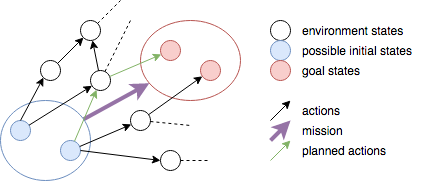
\includegraphics[scale=0.40]{img/env_graph}
\end{figure}

\subsection{Actors (IoT Robots)}

Robots and IoT devices are the executors from which the environment is sensed or modified.

As described previously, the robots are able to do some actions, and will need to execute them in a particular sequence to accomplish a mission.
Since the environment is not completely known, the plan may need to be modified over time.
So, the system making the plan will need a feedback loop to modify it when needed (sense-plan-act ?)
